\documentclass[tikz]{standalone}
\usepackage{pgfplots}
\pgfplotsset{compat=1.15}
\usepackage{mathrsfs}
\usetikzlibrary{arrows,calc}
\usepackage{tkz-euclide}

\usepackage{fp}
\pagestyle{empty}

\definecolor{AngleClr}{rgb}{0,0.39215686274509803,0}
\definecolor{ShapeClr}{rgb}{0.6,0.2,0}

\begin{document}

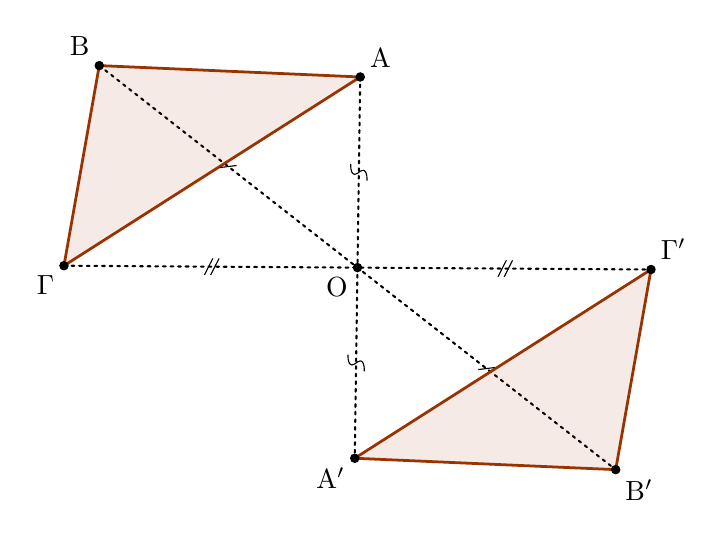
\begin{tikzpicture}[scale=.75]
\tkzSetUpLine[line width=1pt,color=black]
\tkzSetUpPoint[fill=black]

\tkzDefPoint(40:3){A}
\tkzDefPoint(135:3){B}
\tkzDefPoint(205:3){C}
\tkzDefPoint(-30:2.6){O}

\tkzDefPointBy[symmetry=center O](A){} \tkzGetPoint{A'}
\tkzDefPointBy[symmetry=center O](B){} \tkzGetPoint{B'}
\tkzDefPointBy[symmetry=center O](C){} \tkzGetPoint{C'}

\tkzDrawSegments[line width=0.75pt,color=black,dashed,dash pattern=on 1pt off 1.75pt](A,A' B,B' C,C')

\tkzFillPolygon[fill=ShapeClr,fill opacity=0.1](A,B,C)
\tkzFillPolygon[fill=ShapeClr,fill opacity=0.1](A',B',C')
\tkzDrawPolygon[color=ShapeClr](A,B,C)
\tkzDrawPolygon[color=ShapeClr](A',B',C')

\tkzDrawPoints[size=3](A,B,C,A',B',C',O)
\tkzLabelPoint[above right](A){$\rm A$}
\tkzLabelPoint[above left](B){$\rm B$}
\tkzLabelPoint[below left](C){$\rm \Gamma$}
\tkzLabelPoint[below left](O){$\rm O$}

\tkzLabelPoint[below left](A'){$\rm A'$}
\tkzLabelPoint[below right](B'){$\rm B'$}
\tkzLabelPoint[above right](C'){$\rm \Gamma'$}

\tkzMarkSegments[mark=s,size=3](A,O O,A')
\tkzMarkSegments[mark=s|,size=3](B,O O,B')
\tkzMarkSegments[mark=s||,size=3](C,O O,C')

\end{tikzpicture}

\end{document}
